\section{A two-point estimate on spherical cosets}
\label{sec:two-point}

We prove a uniqueness statement that will distinguish the sources in the
spherical-residue filtrations.  Throughout this section, \(T\subseteq S\)
is nonempty and spherical, \(A_Tx_0\) is a fixed right coset, and the
data are capped at an integer \(q\) on \(\partial T\).  The data outside
\(T\) are constant on this coset by
Lemma~\ref{lem:family-proportionality}.  We regard vectors on \(T\) as
vectors on \(\widehat S\) by extension by zero when necessary.

\begin{definition}
\label{def:two-point-candidate}
A \emph{candidate} in \(A_Tx_0\) is a pair
\[
 X=(J,A_Jz),\qquad J\subsetneq T,\qquad z\in A_Tx_0,
\]
with the following properties.  Put \(V=T\setminus J\), and let \(p\)
agree with \(m^q(z)\) outside \(J\) and be harmonic on \(J\).
\begin{enumerate}[label=\textup{(\roman*)}]
\item The data are capped at \(q\) on \(V\).
\item The vector \(a\), defined on \(T\) by
      \(a_i=-(Cp)_i\), is strictly positive on \(V\) and zero on \(J\).
\item For every representative \(y\in A_Jz\) whose data are capped at
      \(q\) on \(T\), one has
      \[
      m_j^q(y)\ge p_j\qquad(j\in J).
      \]
\end{enumerate}
\end{definition}

On the open colors \(V\), the harmonic vector \(p\) retains the actual
layer counts, and condition \textup{(ii)} requires its Cartan rows to be
strictly negative.  On \(J\), the same vector is a harmonic prescription
that condition \textup{(iii)} places below every capped representative's
layer counts.  The source argument in Section~\ref{sec:residues} will
establish these conditions for each source of a residue sublevel.

All three conditions depend only on the indicated coset with its type.
Indeed, changes of representative in \(A_Jz\) change no coordinate
outside \(J\), so they leave \(p\), \(a\), and the cap on \(V\)
unchanged.  The universally quantified set of representatives in
\textup{(iii)} is nonempty: the cap on
\(V\cup\partial T\) gives the cap on \(\partial J\), and
Lemma~\ref{lem:cap-accessibility} supplies a representative capped on
\(J\) as well.  This includes \(J=\varnothing\).

\begin{proposition}
\label{prop:candidate-uniqueness}
There is at most one candidate in \(A_Tx_0\).
\end{proposition}

The proof first compares the harmonic vectors of two candidates by a
tensor estimate.  It then uses right-module tests to turn equality of
those vectors into equality of the cosets.  We develop the tensor
estimate before proving the parabolic detector needed for the second
step.

\subsection{Minimal right complexes and inversion}

For an unfolded vertex \(\ell\in\widetilde T\), let \(U_\ell\) be the
simple top of \(Q_\ell=e_\ell Z\), placed in cochain and internal
degrees zero.  For \(h\in A_T\), consider
\begin{equation}
\label{eq:two-point-right-complex}
 R_\ell(h)=U_\ell\otimes_Z B_h.
\end{equation}
Expansion of a word for \(B_h\) gives a complex with the single term
\(U_\ell\) at placements \((0,0)\), together with shifts of right
projectives \(Q_\beta\), \(\beta\in\widetilde T\).  Here and below a
complex of this form is minimized in the additive category generated
by these graded modules.  This is a Krull--Schmidt category: its
indecomposable terms have finite-dimensional local endomorphism rings.
The cancellation argument of Lemma~\ref{lem:layer-structure} therefore
applies.  The simple cannot cancel against a projective, because the
latter has both a nonzero top and a nonzero token socle.  Consequently
the minimal complex still has exactly this one simple term.

Let
\[
 K^r_{\ell\beta}(h)
\]
denote the number of projective generators of type \(Q_\beta\) and
total generator degree \(r=c+u\) in this minimal complex.  Counts in
different cochain and internal placements with this same sum are
added.  They are well defined by uniqueness of minimal models.

\begin{lemma}
\label{lem:right-duality}
For every \(h\in A_T\), every \(\ell,\beta\in\widetilde T\), and every
integer \(r\),
\begin{equation}
\label{eq:two-point-duality}
 K^r_{\ell\beta}(h)
   =K^{-2-r}_{\beta\ell}(h^{-1}).
\end{equation}
If \(J,J'\subseteq T\), the rows with indices outside
\(\widetilde J'\) are unchanged by left multiplication of \(h\) by
\(A_{J'}\), and the columns with indices outside \(\widetilde J\) are
unchanged by right multiplication of \(h\) by \(A_J\).
\end{lemma}

\begin{proof}
Before minimizing, \(B_h\) has one regular bimodule \(Z\) in placements
\((0,0)\); every other term is a shift of
\(P_\alpha\otimes_{\C}Q_\beta\) with
\(\alpha,\beta\in\widetilde T\).  Tensor products of projective
bimodules remain sums of such terms, since their middle tensor factor
is a graded path space.

No indecomposable summand of the regular bimodule is isomorphic to one
of these projective bimodules.  To see this, decompose \(Z\) according
to the connected components of its unfolded graph.  The regular
bimodule of one component is indecomposable: a decomposition would
give a nontrivial central idempotent, whose degree-zero part would
separate the vertices despite the nonzero arrows between them.  Its
top modulo the left and right radicals consists of the diagonal
simple at every vertex of the component.  The corresponding top of
\(P_\alpha\otimes Q_\beta\) consists of just the single pair
\((\alpha,\beta)\).  Equality of these tops would force a singleton
component and \(\alpha=\beta\).  In that case the regular bimodule has
dimension two, whereas \(P_\alpha\otimes Q_\alpha\) has dimension
four.  Isomorphism is again impossible.  These observations are
unaffected by shifts.  Thus all regular summands remain in the
minimal bimodule complex, and remain only in placements \((0,0)\).

A radical map between projective bimodules is a sum of path tensors
with positive length on at least one side.  The only possible term
with both lengths zero is a scalar map between identical
indecomposable shifted projectives; a nonzero such term would be an
isomorphism modulo the radical and would have been canceled.
Tensoring on the left by \(U_\ell\) kills terms with positive left
length.  Every surviving projective-to-projective differential
therefore has positive right length and is radical.  A map involving
the regular term specializes to a map between \(U_\ell\) and a right
projective, hence is also radical.  There is no differential between
two surviving simple terms, since the regular terms occur only in
cochain degree zero.  It follows that tensoring the minimal bimodule
complex by \(U_\ell\) gives an already minimal right complex.  Its
projective counts are exactly the counts of the corresponding
bimodule terms with first index \(\ell\).

By Lemma~\ref{lem:category-frobenius}, adjoint duality on finite graded
bimodules satisfies
\[
 \Hom_{Z\text{-left}}(M,Z)
       \cong \Hom_\C(M,\C)\langle2\rangle.
\]
It is a contravariant equivalence, preserves additive radicals, and
sends
\[
 P_\ell\otimes Q_\beta
       \quad\longmapsto\quad
 (P_\beta\otimes Q_\ell)\langle-2\rangle.
\]
For complexes it also reverses cochain placements, with the ordinary
cochain dual differential.  Hence a generator at \((c,u)\) on the
left corresponds to one at \((-c,-u-2)\) on the right.  The total
generator degree changes from \(r\) to \(-2-r\).  The adjoint dual
of \(B_h\) is homotopy equivalent to its inverse \(B_{h^{-1}}\), by
Proposition~\ref{prop:twist-action}.  As the dual minimal complex is
still minimal, the preceding specialization proves
\eqref{eq:two-point-duality}.

For \(b\in A_{J'}\) and \(\ell\notin\widetilde J'\), each generator
or inverse generator occurring in \(b\) fixes \(U_\ell\): its
projective evaluation or coevaluation term tensors to zero.  Thus
\[
 U_\ell B_{bh}\simeq U_\ell B_h,
\]
which proves row invariance.  Apply
\eqref{eq:two-point-duality} to \((ha)^{-1}=a^{-1}h^{-1}\), for
\(a\in A_J\), to obtain column invariance.
\end{proof}

\subsection{Normalized right layers}

In a minimal complex \(R_\ell(h)\), keep the usual level \(c+u\) for
each projective generator, and assign the residual simple the
\emph{normalized level} \(-1\).  The actual placements of the simple
remain \((0,0)\).  This assignment has the following elementary
compatibility with differential entries.

A projective-to-projective entry of length \(a\in\{1,2\}\) changes
normalized level by \(1-a\).  A nonzero entry from a projective to
the simple must use the top quotient of \(Q_\ell\).  Its source
placements are \((-1,0)\), so its source also has normalized level
\(-1\).  Conversely, an entry from the simple to a projective uses
the token socle of \(Q_\ell\).  Its target placements are
\((1,-2)\), again of level \(-1\).  Give these two kinds of entries
\emph{effective length one}.  Every differential entry then changes
normalized level by one minus its effective length, and in particular
does not raise normalized level.

At a fixed level, retain the length-one projective entries and these
effective length-one entries.  They give coefficient maps, with the
simple allowed as an additional framing coefficient.  At a
projective vertex \(\beta\), define the \emph{right top} to be the
projective coefficient space modulo the images of all incoming
coefficient maps, including maps from the simple.  Coefficient paths
are nilpotent because their cochain placements strictly increase and
the complex is bounded.

If \(r\) is the highest normalized level of \(R_\ell(h)\), the same
path calculation as in Lemma~\ref{lem:layers-extremal-tests} gives
\begin{equation}
\label{eq:two-point-right-top}
 \dim H^{r+2}(R_\ell(h)e_\beta)
       =\dim\operatorname{top}_\beta(R_\ell(h)^r).
\end{equation}
Indeed, the projective token terms at level \(r\) are the only terms
of total degree \(r+2\).  The incoming images are precisely the
length-one coefficient images tested by the perfect backtrack
pairing, together with the token inclusions from the simple when
\(r=-1\).  A length-two differential reaching such a token from a
length-zero path would have to start at level \(r+1\), which is
absent.  All other possible incoming paths from lower levels would
multiply beyond length two and vanish.  The cohomology in
all higher total degrees vanishes.  Formula
\eqref{eq:two-point-right-top} also applies with a common upper bound
\(r\) for a finite family of these right complexes.

\begin{lemma}
\label{lem:two-point-negative-bound}
Let \(R\) be a minimal complex with a single simple \(U_\ell\) at
\((0,0)\) and shifted right projectives, and let \(r\ge-1\) bound its
normalized levels.  Applying a right inverse twist, and then
minimizing, does not increase this bound.  The same holds for the
product of inverse twists in one color.  At the acted vertex
\(\alpha\), the test complexes satisfy
\begin{equation}
\label{eq:two-point-inverse-test}
 (R D_\alpha)e_\alpha
       \simeq (Re_\alpha)\langle-2\rangle[-1].
\end{equation}
\end{lemma}

\begin{proof}
The inverse bimodule complex is
\[
 D_\alpha=
 [Z\longrightarrow(P_\alpha\otimes Q_\alpha)\langle-2\rangle],
\]
with its second term in cochain degree one.  An old projective
\(Q_\beta\) with placements \((c,u)\), tested against a path of
length \(a\) in \(e_\beta Ze_\alpha\), inserts a copy of
\(Q_\alpha\) with placements
\begin{equation}
\label{eq:two-point-inserted-placements}
 (c+1,u+a-2),
 \qquad\text{of level }c+u+a-1.
\end{equation}
The only insertions that can exceed the old level have \(a=2\), and
then \(\beta=\alpha\).  We cancel all of them simultaneously, keeping
track of the old differential.

Write \(\mathcal E=\operatorname{Tot}(R D_\alpha)\).  In its underlying
bigraded module, let \(A\) be the sum of all old \(Q_\alpha\) terms
in the \(Z\)-column, and let \(B\) be the sum of their inserted
length-two copies.  The copy paired with an old term at \((c,u)\)
lies at \((c+1,u)\).  The token--unit summand of the Frobenius
coevaluation gives an isomorphism
\[
 \Phi=\pi_B d|_A:A\longrightarrow B
\]
of cochain degree one, with signed nonzero scalar identity entries.
The old differential stays within its tensor column and contributes
nothing to this particular block.

Consider
\[
 \mathcal K=A\oplus d(A)\subseteq\mathcal E.
\]
Projection onto \(B\) identifies \(d(A)\) with \(B\), so
\(A\cap d(A)=0\).  The displayed sum is a subcomplex: its
differential maps \(A\) isomorphically to \(d(A)\) and kills
\(d(A)\).  It is contractible, and is a direct summand of the
underlying bigraded module.  Thus the quotient
\(\mathcal E\longrightarrow\mathcal E/\mathcal K\) is a homotopy
equivalence.  More explicitly, if
\(\mathcal E=A\oplus B\oplus W\) as a bigraded module, the quotient
has underlying terms \(W\).  Representing a quotient class by its
\(W\)-component gives the differential
\begin{equation}
\label{eq:two-point-pivot-differential}
 d'_W=d_{WW}-d_{WA}\Phi^{-1}d_{BW}.
\end{equation}
This formula includes any scalar entries that the old differential
induces among the inserted projectives; their vanishing is not
needed.

The remaining projective terms are the old \(Q_\beta\) with
\(\beta\ne\alpha\), and the length-zero and length-one insertions
in \eqref{eq:two-point-inserted-placements}.  Their levels are,
respectively, the old level, the old level minus one, and the old
level.  The original simple remains at normalized level \(-1\).
If \(\alpha=\ell\), the simple also inserts a projective with
placements \((1,-2)\), of level \(-1\); if \(\alpha\ne\ell\), it
inserts nothing.  All surviving terms have level at most \(r\).
Further minimization removes summands without introducing new ones,
so preserves this bound.  Applying this argument successively to the
orthogonal vertices of a color proves the color statement.

Finally, the inverse of the right-hand test-shift formula for the
positive twist in Lemma~\ref{lem:positive-layer} is
\eqref{eq:two-point-inverse-test}.  Equivalently, it follows by
canceling the token--unit component of \(D_\alpha e_\alpha\).
Its total shift is \(-2+1=-1\), so in particular
\[
 H^t((R D_\alpha)e_\alpha)
       \cong H^{t+1}(Re_\alpha).
\]
The shift formula holds for the nonprojective simple input as well,
since the cancellations are bimodule homotopies before tensoring.
\end{proof}

\subsection{The highest pair in the tensor filtration}

Compare two candidates, denoted by
\[
 (J,A_Jz),\quad (J',A_{J'}z'),
 \qquad V=T\setminus J,\quad V'=T\setminus J',
\]
and use \(p,a\) and \(p',a'\) for their harmonic vectors and
strictly positive open-color vectors.  By cap accessibility inside
\(J\), choose \(z\) capped at \(q\) on \(T\).  The initial
representative \(z'\) need only have the prescribed cap on \(V'\).
Set
\[
 h=z'z^{-1}\in A_T,
 \qquad R_\ell=R_\ell(h)\quad(\ell\in\widetilde V').
\]
Give the row \(\ell=(i,L)\) weight \(a'_i w_L\), and give each
left-family member \(E_{L'}(z)\) weight \(w_{L'}\), independently.
All these weights are positive.  Since
\[
 R_\ell\otimes_Z E_{L'}(z)
       \simeq U_\ell B_h B_zP_{o,L'}
       \simeq U_\ell E_{L'}(z'),
\]
the weighted total cohomology in degree \(d\) has dimension
\begin{equation}
\label{eq:two-point-actual-homology}
 D_0\sum_{i\in V'}a'_i m_i^d(z'),
 \qquad D_0=\sum_L w_L^2.
\end{equation}
Here tensoring a minimal left complex with \(U_\ell\) kills its
radical differential and counts its generators of type \(\ell\).
Summing first over \(L'\) gives \(w_Lm_i^d(z')\), and summing the
row weights gives \eqref{eq:two-point-actual-homology}.  In particular
all these tensor complexes have zero cohomology above \(q\).

Let \(r\ge-1\) be the highest normalized level appearing in the
finite right family.  Write \(N\) for its coefficient data at that
level, retaining the row index, and let
\[
 M_{L'}=Y_{L'}^q(z),\qquad M=(M_{L'})_{L'}.
\]
We define a three-term vector-space complex for each row and left
member.  Its length-zero terms are tensors of right and left
coefficients with an intervening length-zero path, its length-two
terms use tokens, and its length-one terms use arrows.  If \(r=-1\),
the simple-against-projective tensors are also placed in length one.
The differential is the length-one part of the tensor differential.
Write \(H_j(N,M)\) for the resulting cohomology in length
\(j\in\{0,1,2\}\), keeping the family indices when needed.  Its
weighted dimension, denoted \(\dim_{\mathrm{wt}}\), uses the two
independent weights just specified.

\begin{lemma}
\label{lem:two-point-tensor-filtration}
With these definitions,
\begin{equation}
\label{eq:two-point-highest-tensor}
 H_2(N,M)=0,
 \qquad
 H_1(N,M)\text{ survives in actual total degree }r+q+1.
\end{equation}
Moreover, at every unfolded projective vertex \(\beta\), the
length-two cokernel surjects onto the tensor product of the right
and left top quotients at \(\beta\).  Consequently, if a right top
at level \(r\) occurs in a color \(j\in J\), then all the
left-family tops at level \(q\) in that color vanish.
\end{lemma}

\begin{proof}
Filter the entire vector complex
\(R_\ell\otimes_Z E_{L'}(z)\) by middle path lengths zero, one, and
two, assigning length one to a simple tensor.  Minimal projective
differentials have positive path length.  The map from a projective
to a simple sends a length-zero tensor to the assigned length-one
tensor and kills positive middle paths; the map from the simple to
a projective sends its assigned length-one tensor to a token tensor.
A left radical differential tensored with a right simple is zero.
Thus every differential strictly increases this filtration index.

For a right projective generator at \((c,u)\), a left generator at
\((c',u')\), and a middle path of length \(a\), the total degree is
\[
 (c+u)+(c'+u')+a.
\]
For the simple tensor it is \(c'+u'=(-1)+(c'+u')+1\), the same rule
with the normalized right level.  The first differential of the
filtration increases length by one and preserves each pair of
levels.  Its cohomology at the pair \((r,q)\) is precisely
\(H_j(N,M)\).  With only three length columns, the only possible
remaining differential goes from length zero to length two.
Accordingly, every middle class survives to the associated graded
of actual cohomology.

Every right projective has its vertex in \(\widetilde T\).
The tensor \(Q_\beta\otimes_Z P_\gamma=e_\beta Ze_\gamma\) is
nonzero only if \(\gamma=\beta\) or \(\gamma\) is a neighbor of
\(\beta\).  A simple tensor is nonzero only at its own vertex in
\(\widetilde T\).  Hence every nonzero term of the entire tensor
complex uses a left color in \(T\cup\partial T\), where the cap is
\(q\).  Layers above \(q\) outside this set give zero tensor terms.

A secondary differential into length two at \((r,q)\) would start
in length zero at a pair whose level sum is \(r+q+1\): the
differential raises actual total degree by one while raising length
by two.  Such a pair is absent, since the right level is at most
\(r\) and every relevant left level is at most \(q\).  Thus
\(H_2(N,M)\) survives as well.  Its total degree is
\(r+q+2>q\), so \eqref{eq:two-point-actual-homology} forces it to be
zero.  The middle degree is \(r+q+1\), proving
\eqref{eq:two-point-highest-tensor}.

For the last assertion, project the token tensors at \(\beta\) to
the tensor product of the two coefficient spaces modulo their
incoming images, and send all other token tensors to zero.
Every incoming length-one boundary has, at \(\beta\), an incoming
coefficient on at least one side.  The projection therefore
annihilates boundaries and is surjective onto the tensor product of
the two top quotients.  If a right top at a vertex of color \(j\)
is nonzero, \(H_2(N,M)=0\) forces the left top at that same vertex
to be zero for every family member.  By
Lemma~\ref{lem:family-proportionality}, a top occurring anywhere in
a color of the left family occurs at every unfolded label of that
color in some member.  Hence no left-family top in color \(j\)
can occur.
\end{proof}

Figure~\ref{fig:filtrations} records the two excluded incoming sources at
\((r,q)\) and the permanent middle column.

\begin{figure}[tbp]
  \centering
  {\small
    Linear part: $C_0\xrightarrow{d_1}C_1\xrightarrow{d_1}C_2$,
    \quad $H_a=H^a(C_\bullet,d_1)$.\par}
  \medskip
  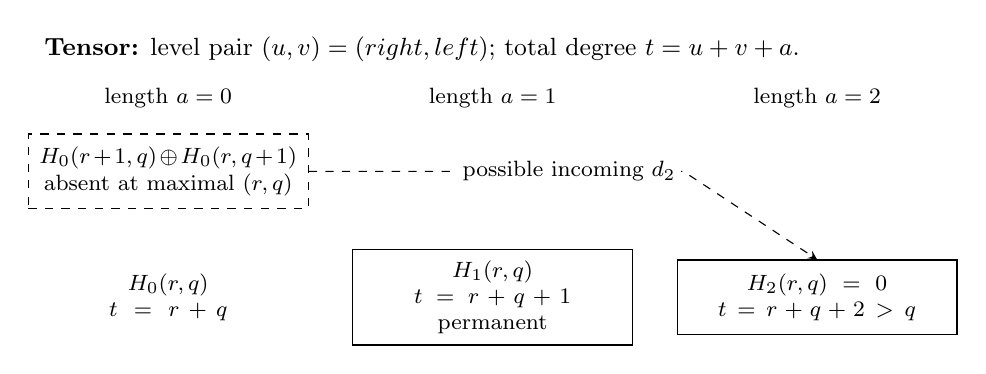
\begin{tikzpicture}[
      x=.01\linewidth,y=1cm,
      every node/.style={font=\footnotesize,align=center},
      term/.style={text width=.27\linewidth,inner sep=4pt},
      permanent/.style={term,draw,semithick,minimum height=.95cm},
      endpoint/.style={term,draw,thin,minimum height=.95cm},
      excluded/.style={term,draw,dashed,thin,minimum height=.95cm},
      differential/.style={->,thin,>=stealth}
    ]
    \node[anchor=west,align=left,font=\small] at (-14,0)
      {\textbf{Tensor:} level pair $(u,v)=(\text{right},\text{left})$;
        total degree $t=u+v+a$.};
    \node at (0,-.62) {length $a=0$};
    \node at (34,-.62) {length $a=1$};
    \node at (68,-.62) {length $a=2$};
    \node[excluded] (tensor-sources) at (0,-1.55)
      {$H_0(r+1,q)\oplus H_0(r,q+1)$\\
        absent at maximal $(r,q)$};
    \node[term] (tensor-zero) at (0,-3.15)
      {$H_0(r,q)$\\$t=r+q$};
    \node[permanent] (tensor-middle) at (34,-3.15)
      {$H_1(r,q)$\\$t=r+q+1$\\permanent};
    \node[endpoint] (tensor-two) at (68,-3.15)
      {$H_2(r,q)=0$\\$t=r+q+2>q$};
    \draw[differential,dashed] (tensor-sources.east)
      -- (54,-1.55) -- (tensor-two.north);
    \node[fill=white,inner sep=2pt] at (42,-1.55)
      {possible incoming $d_2$};

  \end{tikzpicture}
  \caption{The tensor length filtration at the highest contributing pair
    $(r,q)$.  The right normalized level is at most $r\ge-1$, and every
    contributing left color is in $T\cup\partial T$, where the cap is $q$.
    The only possible secondary differential is $d_2:0\to2$, so the middle
    classes are permanent.  Its two possible incoming sources at $(r,q)$
    are absent; hence the length-two classes also survive.  Their actual
    degree $r+q+2>q$ forces $H_2(r,q)=0$.  A residual right simple has
    normalized level $-1$ and assigned length $1$, which preserves the
    total-degree formula.  The dashed arrow marks an excluded possibility.
    Family and bidegree indices are suppressed.}
  \label{fig:filtrations}
\end{figure}


\begin{lemma}
\label{lem:two-point-remove-tops}
By replacing \(z\) within \(A_Jz\), preserving the cap on \(T\), one
can arrange that the highest normalized right layer has no right
top at any vertex of \(\widetilde J\).
\end{lemma}

\begin{proof}
Suppose a right top at the current highest level \(r\) occurs in
color \(j\in J\).  Lemma~\ref{lem:two-point-tensor-filtration} shows
that the left-family top in this color at level \(q\) vanishes.
The positive operation \(F_j\) therefore preserves the cap on
\(T\cup\partial T\), by Lemma~\ref{lem:cap-accessibility} applied
with spherical set \(T\).  Replace
\[
 z\longmapsto\sigma_jz,
 \qquad h\longmapsto h\sigma_j^{-1},
 \qquad R_\ell\longmapsto R_\ell B_{\sigma_j}^{-1}.
\]
The candidate, its harmonic vector \(p\), and the exterior cap are
unchanged.  The tensor products still compute the same complexes
\(U_\ell E_{L'}(z')\).  By
Lemma~\ref{lem:two-point-negative-bound}, the new maximum normalized
level is at most \(r\).  Thus the vanishing of the left top needed
to license the next move follows anew from
Lemma~\ref{lem:two-point-tensor-filtration}.

At a fixed value of \(r\), the sequence of chosen colors is reduced
in \(W_J\).  To prove this, let \(w\) be the reduced word already
chosen at this level.  If a color \(j\) were a right descent of
\(w\), a reduced expression for \(w\) could end in \(j\).
Matsumoto moves give the same negative Artin word in this
expression.  Each intermediate negative operation preserves the
upper bound \(r\), regardless of the expression.  The final inverse
operation in color \(j\) lowers the total test degrees in that
color by one.  Before it, every test above \(r+2\) vanishes; after
it, every test at \(r+2\) in color \(j\) therefore vanishes.
Formula~\eqref{eq:two-point-right-top} excludes a right top there.
A color selected for a nonzero right top must consequently be an
ascent, proving the assertion by induction on the number of moves.

The length of a reduced word in \(W_J\) is bounded by the length of
its longest element.  Therefore at a fixed \(r\) the procedure
either removes all the indicated tops or lowers the maximum level
after finitely many steps.  The maximum is an integer bounded below
by \(-1\), because the residual simples remain.  There are only
finitely many possible decreases from its initial value.  The
procedure terminates with the desired representative.  If
\(J=\varnothing\), no move is needed.
\end{proof}

\FloatBarrier
\subsection{Subrepresentations and the Euler estimate}

Use the representative supplied by
Lemma~\ref{lem:two-point-remove-tops}, and retain the notation
\(r,N,M\) for its highest right layer and left layer at \(q\).
Put
\[
 m=m^q(z),\qquad e=m-p.
\]
The vector \(e\) is supported on \(J\).  The cap on
\(T\cup\partial T\), together with the universal condition in
Definition~\ref{def:two-point-candidate}, verifies the hypotheses of
Proposition~\ref{prop:convex-subobjects} for \(A_Jz\).  Indeed, on
this coset the cap on \(T\setminus J\) is fixed, so a representative
capped on \(J\cup\partial J\) is also capped on \(T\).
Consequently \(e_J\) belongs to the convex hull of folded dimension
vectors \(s_J\) of families
\begin{equation}
\label{eq:two-point-subfamilies}
 \mathcal S_{L'}\subseteq M_{L'}
\end{equation}
of graded layer subrepresentations supported on \(\widetilde J\).
Their weighted dimensions have the form \(\phi s\), with \(s\)
zero outside \(J\).

\begin{lemma}
\label{lem:two-point-subrepresentation-tensor}
For every family \(\mathcal S\subseteq M\) in
\eqref{eq:two-point-subfamilies},
\begin{equation}
\label{eq:two-point-subrepresentation-homology}
 H_2(N,\mathcal S)=0,
 \qquad
 H_0(N,\mathcal S)\hookrightarrow H_0(N,M).
\end{equation}
\end{lemma}

\begin{proof}
The inclusion in degree zero follows from the inclusion of the
length-zero vector spaces and compatibility of the length-one
differentials.  Since there is no incoming term of negative length,
their degree-zero cohomologies are kernels, and kernel inclusion
gives the asserted injection.

For the degree-two assertion, work first with a single right row
and a single left subrepresentation, and retain homogeneous
coefficient spaces in their cochain gradings.  At every projective
vertex of \(\widetilde J\), vanishing of the right top says that
every right coefficient is a sum of incoming coefficient images,
from projective vertices or from the framing simple.  Iterating
this statement expresses coefficients in \(\widetilde J\) using
ones outside \(\widetilde J\) or in the simple: along an incoming
projective path the predecessor cochain placement is smaller by
one, and these placements are bounded below.

We make this iteration in the cokernel of the length-one
differential, rather than in the coefficient spaces alone.  Suppose
an incoming right coefficient at \(\beta\) comes from a homogeneous
coefficient at \(\gamma\), through a length-one map
\(Q_\gamma\to Q_\beta\).  Choose a middle path in
\(e_\gamma Z^1e_\beta\) dual to this arrow under the perfect
backtrack pairing.  Tensor this middle path with the coefficient
at \(\gamma\) and any homogeneous left coefficient in
\(\mathcal S_\beta\).  Its differential has two possible token
contributions.  The contribution at \(\beta\) is the selected
incoming right coefficient, tensored with the unchanged left
coefficient.  The contribution at \(\gamma\) is the original right
coefficient tensored with the corresponding left-arrow image, with
the ordinary cochain sign.  The dual path can be normalized so that
the first coefficient is one.  Hence, modulo length-two boundaries,
the token tensor at \(\beta\) is equal, up to a nonzero scalar and
sign, to the latter token tensor at \(\gamma\).

The new left coefficient lies in \(\mathcal S_\gamma\), since
\(\mathcal S\) is closed under the left coefficient maps.  Varying
the dual middle path tests every incoming arrow coefficient by
nondegeneracy of the pairing, including when an arrow space has
dimension greater than one.  Thus this substitution accounts for
the full span of incoming images.  Each substitution decreases the
right cochain placement by one and increases the left placement by
one, so the represented total degree is unchanged and the
substitution process terminates.

If it terminates at a projective vertex outside \(\widetilde J\),
the left coefficient is zero.  If an incoming coefficient comes
from the simple, its tensor with the same left coefficient is
itself an assigned length-one input.  The right differential sends
that tensor to exactly the token-inclusion image in question.  Its
left differential is zero because tensoring a radical left map
with a right simple gives zero.  Such a token tensor is therefore
already a boundary.  Every length-two generator is a sum of the
tensors just treated, so the cokernel vanishes.  This proves the
first assertion row by row and member by member, hence for the
families as well.
\end{proof}

Define the folded nonnegative vector \(n\), supported on \(T\), by
\begin{equation}
\label{eq:two-point-right-weight}
 n_j=\frac1{D_0}\sum_H w_H
       \sum_{i\in V'}\sum_L a'_i w_L
                K^r_{(i,L),(j,H)}(h)
       \qquad(j\in T).
\end{equation}
For any left-layer family of weighted dimension \(\phi y\), the
weighted Euler characteristic of its length complex with \(N\),
divided by \(D_0\), is
\begin{equation}
\label{eq:two-point-euler}
 \chi(n,y)=n^{\mathsf t}Cy
       -\mathbf1_{\{r=-1\}}(a')^{\mathsf t}y_T.
\end{equation}
Here is the count explicitly.  If
\[
 N_\beta^{\mathrm{wt}}
      =\sum_{i\in V'}\sum_L a'_i w_L K^r_{(i,L),\beta}(h),
\]
the projective part of the unnormalized count is
\[
 \sum_{\beta,\gamma}
       N_\beta^{\mathrm{wt}}\widetilde C_{\beta\gamma}(\phi y)_\gamma
   =\sum_{j,H}N_{(j,H)}^{\mathrm{wt}}w_H(Cy)_j
   =D_0 n^{\mathsf t}Cy.
\]
The two diagonal paths, of lengths zero and two, give diagonal
coefficient two; the middle arrows give minus adjacency.  We used
\(\widetilde C\phi=\phi C\) in the first equality.  If \(r=-1\),
the residual simples also occur at this level.  Their length-one
contribution is
\[
 -\sum_{i\in V'}\sum_L a'_i w_L\,(w_Ly_i)
      =-D_0(a')^{\mathsf t}y_T.
\]
No simple is present in \(N\) when \(r>-1\).  This proves
\eqref{eq:two-point-euler}, including its normalization and sign.

\begin{lemma}
\label{lem:two-point-euler-estimate}
At the representative with no highest right tops on \(J\),
\begin{equation}
\label{eq:two-point-estimate}
 \frac1{D_0}\dim_{\mathrm{wt}}H_1(N,M)
       \ge n_T^{\mathsf t}a
              +\mathbf1_{\{r=-1\}}(a')^{\mathsf t}p_T.
\end{equation}
\end{lemma}

\begin{proof}
For a family \(\mathcal S\) with folded dimension \(s\),
Lemma~\ref{lem:two-point-subrepresentation-tensor} and the Euler
identity give
\[
 \chi(n,s)
  =\frac{\dim_{\mathrm{wt}}H_0(N,\mathcal S)
             -\dim_{\mathrm{wt}}H_1(N,\mathcal S)}{D_0}
  \le\frac{\dim_{\mathrm{wt}}H_0(N,M)}{D_0}.
\]
The right side is independent of the chosen subfamily.  Since
\(e\) is a convex combination of these \(s\), and
\(\chi(n,\cdot)\) is linear, the same upper bound holds for
\(\chi(n,e)\).  On the other hand,
Lemma~\ref{lem:two-point-tensor-filtration} gives
\[
 \chi(n,m)
   =\frac{\dim_{\mathrm{wt}}H_0(N,M)
             -\dim_{\mathrm{wt}}H_1(N,M)}{D_0}.
\]
Subtracting yields
\[
 \frac1{D_0}\dim_{\mathrm{wt}}H_1(N,M)
    \ge\chi(n,e)-\chi(n,m)=-\chi(n,p).
\]
Finally, \(n\) is supported on \(T\), and \((Cp)_T=-a\).
Equation~\eqref{eq:two-point-euler} therefore turns the right side
into the expression in \eqref{eq:two-point-estimate}.
\end{proof}

\subsection{A spherical parabolic detector}

The tensor estimate is now available.  In the final comparison it will
force the harmonic vectors of two candidates to agree; to identify their
cosets as well, we need to recover parabolic membership from a vanishing
block of the right-projective counts \(K^r_{\ell\beta}\).

We need to reflect positive last-letter divisibility through the
finite unfolding.  Recall that a \emph{simple} positive element in a
finite-type Artin monoid is a reduced-word lift of an element of the
Coxeter group \(W_T\).
The finite-type monoid facts in
Theorem~\ref{thm:topology-finite-monoid} imply that the greatest simple
right divisor of a positive element \(b\) exists: it is its right gcd
with the Garside element.  Write it as \(t(b)\).

\begin{lemma}
\label{lem:two-point-greedy}
For nonidentity simple elements \(d_1,\ldots,d_k\), the factorization
\(d_1\cdots d_k\) is obtained by repeatedly extracting the greatest
simple suffix if and only if
\begin{equation}
\label{eq:two-point-greedy-condition}
 D_R(d_i)\subseteq D_L(d_{i+1})\qquad(1\le i<k).
\end{equation}
Here the descent sets are those of the corresponding elements of
the Coxeter group.  Consequently, if an unfolded vertex right-divides the
unfolding of a positive element of \(A_T^+\), its original color
right-divides that positive element.
\end{lemma}

\begin{proof}
An atom \(s\) right-divides a simple element \(d\) exactly when
\(s\in D_R(d)\), and \(sd\) is simple exactly when
\(s\notin D_L(d)\).  If the inclusion in
\eqref{eq:two-point-greedy-condition} fails, an atom in its difference
can be transferred from the end of \(d_i\) to the beginning of
\(d_{i+1}\), giving a larger simple suffix of the corresponding
prefix.  This proves necessity.

For sufficiency, induct on prefixes.  Suppose
\(P=d_1\cdots d_{j-1}\) has greatest simple suffix \(d_{j-1}\), and
let \(g=t(Pd_j)\).  Since \(d_j\) is a simple suffix, it right-divides
\(g\); write \(g=cd_j\).  If \(c\ne1\), choose a final atom of
\(c\), so \(c=c's\).  The element \(sd_j\), being a factor of the
simple element \(g\), is simple.  Also \(Pd_j=bg=bc d_j\) for some
positive \(b\), so cancellation gives \(P=bc\).  Thus \(s\)
right-divides \(P\).  Since an atom is simple, it right-divides
\(t(P)=d_{j-1}\).  We have obtained
\(s\in D_R(d_{j-1})\) and \(s\notin D_L(d_j)\), a contradiction.
Therefore \(g=d_j\), completing the induction.  Removing the final
factor successively gives the asserted greedy extraction.

Now take the greedy factorization of a positive original element.
Lemma~\ref{lem:finite-unfolding} says that reduced-word lifts remain
simple after unfolding, and that both descent sets become their full
color preimages.  Thus the unfolded factors satisfy
\eqref{eq:two-point-greedy-condition} and form the unfolded greedy
factorization.  Every extractable final atom of the unfolded element
right-divides its greatest simple suffix, hence is a right descent
of the last unfolded factor.  Descent reflection supplies its color
as a right descent of the last original factor.  That original atom
therefore right-divides the original positive element.
\end{proof}

The following detector uses successive common-divisor removal, as in
the proof of Brav--Thomas~\cite[Theorem~3.1]{BravThomas2011}.
Here the vanishing block of a family of right-simple tests yields a
specific parabolic subgroup; the unfolding step needed to recover
original colors is Lemma~\ref{lem:two-point-greedy}.

\begin{lemma}
\label{lem:parabolic-detection}
Let \(h\in A_T\) and \(\varnothing\ne V\subseteq T\).  If
\begin{equation}
\label{eq:two-point-zero-block}
 K^r_{\ell\beta}(h)=0
 \qquad
 (r\in\Zbb,\ \ell,\beta\in\widetilde V),
\end{equation}
then \(h\in A_{T\setminus V}\).
\end{lemma}

\begin{proof}
Fix \(\ell\in\widetilde V\).  The only right projective admitting a
nonzero map to or from \(U_\ell\) is \(Q_\ell\): a map to the simple
uses its top quotient, and a map from the simple uses its token
socle.  Condition~\eqref{eq:two-point-zero-block} excludes this
projective from \(R_\ell(h)\).  Its simple term therefore splits off
as a complex.  Tensoring with \(B_h\) is a homotopy equivalence and
preserves indecomposability.  Since \(U_\ell\) is indecomposable, the
remaining projective summand must be zero in the homotopy category.
It follows that
\[
 U_\ell B_h\simeq U_\ell\qquad(\ell\in\widetilde V).
\]

Use finite-type fractions to write \(h=h_1h_2^{-1}\) with
\(h_1,h_2\in A_T^+\).  On setting
\(U_V=\bigoplus_{\ell\in\widetilde V}U_\ell\), the preceding
equivalences give
\begin{equation}
\label{eq:two-point-equal-positive}
 U_V B_{h_1}\simeq U_V B_{h_2}.
\end{equation}
For a bounded right complex \(R\), use the height
\[
 \max\{t:H^t(Re_\beta)\ne0
                    \text{ for some }\beta\in\widetilde T\}
\]
from Lemma~\ref{lem:top-divisor}, with total cohomological degree as
there.  Its value on \(U_V\) is zero.  A positive word avoiding
\(V\) fixes \(U_V\).  If a positive word contains a color of \(V\),
all operations before its first such occurrence fix \(U_V\), and
that first occurrence acts on a highest test and raises the height.
The height cannot subsequently decrease.  Thus the final height is
positive exactly when the word contains a color of \(V\).

If the common height in \eqref{eq:two-point-equal-positive} is
positive, any vertex with highest cohomology gives, by the right
version of Lemma~\ref{lem:top-divisor}, an extractable final atom of
both unfolded positive words.  Lemma~\ref{lem:two-point-greedy}
supplies a common extractable original color \(s\).  Write
\(h_i=g_i\sigma_s\), and tensor
\eqref{eq:two-point-equal-positive} on the right by
\(B_{\sigma_s}^{-1}\).  This gives the same equality with \(g_i\)
in place of \(h_i\), while
\[
 h_1h_2^{-1}=g_1\sigma_s\sigma_s^{-1}g_2^{-1}=g_1g_2^{-1}.
\]
The sum of positive lengths decreases by two.  Repetition therefore
terminates with common height zero.  Both remaining positive words
then avoid \(V\), so their fraction lies in \(A_{T\setminus V}\).
\end{proof}

\subsection{Equality of candidates}

\begin{proof}[Proof of Proposition~\ref{prop:candidate-uniqueness}]
Suppose two candidates are given, and use the notation above.  Carry
out the top-removal procedure for the first candidate, with the
second supplying the positive row weights.  If its final highest
normalized right level satisfies \(r>-1\), that level contains a
nonzero projective coefficient and no framing simple.  It must
contain a nonzero coefficient in \(\widetilde V\).  Indeed, if it
were supported entirely on \(\widetilde J\), vanishing of all its
right tops there would express every coefficient using incoming
ones with strictly smaller cochain placement.  Boundedness would
force every coefficient to be zero.

All row weights are strictly positive.  A nonzero coefficient in
\(\widetilde V\) consequently gives \(n_i>0\) for some \(i\in V\).
Since \(a_i>0\) there, \(n_T^{\mathsf t}a>0\).
Equation~\eqref{eq:two-point-estimate} then gives nonzero middle
cohomology.  It survives in actual total degree \(r+q+1>q\),
contradicting \eqref{eq:two-point-actual-homology}.  We conclude that
\(r=-1\).

At this level the surviving middle cohomology lies in total degree
\(q\), so its weighted dimension is at most that of actual
cohomology there.  Since \(a'\) is supported on \(V'\), where
\(p'_i=m_i^q(z')\), equations
\eqref{eq:two-point-actual-homology} and
\eqref{eq:two-point-estimate} give
\begin{equation}
\label{eq:two-point-forward}
 (a')^{\mathsf t}(p'_T-p_T)
       \ge n_T^{\mathsf t}a\ge0.
\end{equation}
Interchanging the candidates and repeating the argument gives
\begin{equation}
\label{eq:two-point-reverse}
 a^{\mathsf t}(p_T-p'_T)\ge0.
\end{equation}
The two algorithms may choose different representatives.  The
vectors \(p,p',a,a'\), being data of the candidate cosets, are
unchanged by these choices.

The exterior coordinates of \(p\) and \(p'\) outside \(T\) agree.
Put \(\delta=p'_T-p_T\).  Then
\[
 a'-a=-C_T\delta.
\]
The sum of the left sides of \eqref{eq:two-point-forward} and
\eqref{eq:two-point-reverse} is therefore
\[
 (a'-a)^{\mathsf t}\delta
       =-\delta^{\mathsf t}C_T\delta.
\]
Both summands are nonnegative, whereas \(C_T\) is positive definite.
It follows that \(\delta=0\) and equality holds throughout.
Thus \(p=p'\), \(a=a'\), and
\[
 V=\{i\in T:a_i>0\}=V',\qquad J=J'.
\]
In particular the nonnegative term \(n_T^{\mathsf t}a\) in
\eqref{eq:two-point-forward} is zero.

It remains to identify the cosets, rather than just their numerical
data.  Fix the comparison element \(h_0=z'z^{-1}\) using any initial
representatives of the two candidates.  Replacing these by \(bz\)
and \(cz'\), with \(b\in A_J\) and \(c\in A_{J'}\), changes it to
\[
 c h_0 b^{-1}.
\]
By Lemma~\ref{lem:right-duality}, the block with row indices in
\(\widetilde V'\) and column indices in \(\widetilde V\) is
invariant under all such changes.  After the equality just proved,
this is the same block \(\widetilde V\times\widetilde V\) in both
directions.

In the forward comparison no right projective generator has degree
above \(-1\).  At degree \(-1\), the equality
\(n_T^{\mathsf t}a=0\), formula~\eqref{eq:two-point-right-weight},
and strict positivity of all its weights imply
\[
 K^{-1}_{\ell\beta}=0
       \qquad(\ell,\beta\in\widetilde V).
\]
Indeed every summand contributing to a column color in \(V\) has
a positive coefficient, and all counts are nonnegative.  By block
invariance, the fixed block for \(h_0\) is therefore zero in every
degree \(d\ge-1\).  The reverse comparison proves that the same
block for \(h_0^{-1}\) is zero for all \(d\ge-1\), irrespective of
the representatives chosen in that direction.  Formula
\eqref{eq:two-point-duality} transposes these latter vanishings into
vanishing of the block for \(h_0\) in all degrees \(d\le-1\).
Together the two ranges give
\[
 K^d_{\ell\beta}(h_0)=0
       \qquad(d\in\Zbb,\ \ell,\beta\in\widetilde V).
\]
Lemma~\ref{lem:parabolic-detection} gives
\(h_0\in A_{T\setminus V}=A_J\).  Thus
\(z'=h_0z\) and \(A_Jz'=A_Jz\), proving equality of the two
candidates.
\end{proof}
